\section{Desarrollo interfaz de control del Datapath - \texttt{dpctl}}
\label{sec:dpctl}

En esta sección se va a estudiar el funcionamiento interno de la herramienta \texttt{dpctl}\footnote{\url{https://github.com/CPqD/ofsoftswitch13/blob/master/utilities/dpctl.c}}, la cual se utiliza para gestionar y controlar el plano de datos de software switch BOFUSS. La motivación de esta sección radica en el desarrollo realizado para adaptar su funcionamiento a raíz de encontrar serios problemas en su interfaz de comandos. Dichos problemas e incompatibilidades llevan registrados en varios \textit{issues}\footnote{\url{https://github.com/mininet/mininet/issues/745}}\footnote{\url{https://github.com/CPqD/ofsoftswitch13/issues/288}}\footnote{\url{https://github.com/mininet/mininet/issues/628}} desde el 2018 tanto en Mininet como en el repositorio de \gls{bofus}, lo que hacía ingestionable la comprobación del correcto funcionamiento del software switch modificado.\\
\\
La problemática principal que se ha encontrado a la hora de hacer \textit{debug} sobre la implementación del \gls{bofus}, cuando se deseaba obtener las tablas de los flujos que se deberían haber instalado en el switch, sin embargo, estas no aparecen.\\
\\

% fig
\begin{figure}[ht]
    \centering
    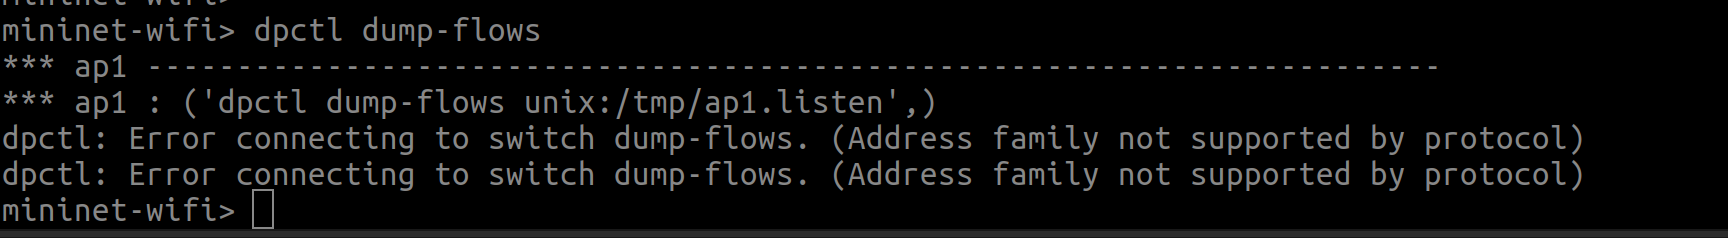
\includegraphics[width=0.8\textwidth]{archivos/img/dev/dpctl_1.png}
    \caption{Error en la interfaz de control del \glsentryshort{bofus} desde Mininet-WiFi}
    \label{fig:dpctl_1}
\end{figure}

En una primera instancia, procedimos a verificar la existencia y ubicación correcta de los dos sockets UNIX mencionados en el lanzamiento del plano de datos y control del switch (ver Bloque de código \ref{code:bofussLaunch}). Se constató que efectivamente se generaron dichos descriptores y que disponían de los permisos adecuados. Como se puede observar en los comandos previos, se especifican dos sockets UNIX. Uno de ellos, denominado \texttt{/tmp/ap1}, se destina a la intercomunicación entre el plano de datos y el plano de control, mientras que el segundo, \texttt{/tmp/ap1.listen}, se utiliza para la gestión interna, tal como se señala en la documentación pertinente del switch. Indagando más allá, se ha tomado la decisión de llevar a cabo el lanzamiento de la herramienta desde fuera del entorno de Mininet-WiFi. Esta medida se ha adoptado con el fin de descartar la posibilidad de que el problema surgiera a raíz de un error interno en la forma en que el emulador invoca la herramienta de control. En consecuencia, se procedió a ejecutar la herramienta directamente desde la terminal, y tal como se había presupuesto, se vió que se obtiene el mismo comportamiento (Ver Figura \ref{fig:dpctl_2}).\\

% fig
\begin{figure}[ht]
    \centering
    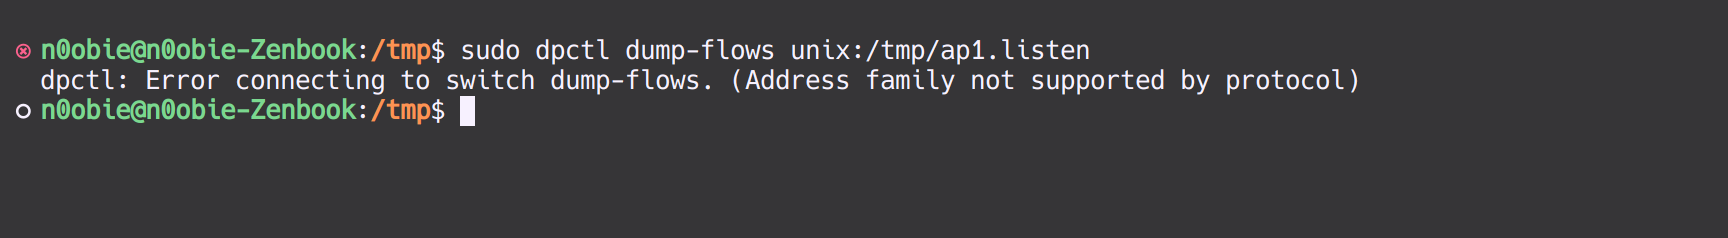
\includegraphics[width=\textwidth]{archivos/img/dev/dpctl_2.png}
    \caption{Error en la interfaz de control del \glsentryshort{bofus}}
    \label{fig:dpctl_2}
\end{figure}


Inicialmente, se asumió que la herramienta en cuestión había sido desarrollada por Eder, basándose en el hecho de que en el repositorio de \gls{bofus} se encuentran tanto las fuentes\footnote{\url{https://github.com/CPqD/ofsoftswitch13/blob/master/utilities/dpctl.c}} del binario compilado e instalado, como la documentación asociada\footnote{\url{https://github.com/CPqD/ofsoftswitch13/blob/master/utilities/dpctl.8.in}}, es decir, las páginas de manual o \textit{man pages}. Sin embargo, esta suposición resultó ser equivocada. En realidad, la herramienta es heredada de Stanford y data del año 2008. Se llegó a esta conclusión al percatarse de que se instalan las páginas de manual de la versión antigua de la herramienta, y en ellas se referencia a la implementación primigenea.\\
\\
Consultando la documentación de ambas herramientas, la original mediante \texttt{man dpctl}, y la modificada, mediante \texttt{dpctl -h}, se puedo apreciar que la sintaxis era completamente diferente. A continuación, en el bloque \ref{code:dpctlDiff} se indican las diferencias más notables en la CLI.

\begin{lstlisting}[language= bash, style=Consola, caption={Diferencias en las herramientas dpctl},label=code:dpctlDiff]
    # [Original] Herramienta dpctl 
    sudo dpctl CMD [SW]

    # [Modificada] Herramienta dpctl 
    sudo dpctl [SW] CDM 
\end{lstlisting}
\vspace{0.5cm}

Es evidente que la sintaxis ha experimentado cambios significativos. Se observa claramente cómo se han intercambiado los parámetros de comando y de identificación del switch en cuestión. Sin embargo, los cambios no se limitan solo a la reorganización de los parámetros, sino que también se han modificado los comandos disponibles en la herramienta.\\
\\
Un ejemplo ilustrativo es el comando \texttt{dump-flows}, que es ampliamente reconocido y utilizado en la documentación de Mininet para recopilar información sobre los flujos instalados en la lógica interna del switch. Si examinamos el código fuente de la herramienta original, podemos confirmar que existe una función específica para proporcionar dicha funcionalidad. La función en cuestión se encuentra en el siguiente enlace:

\begin{itemize}
    \item \href[]{https://github.com/mininet/openflow/blob/master/utilities/dpctl.c#L1114}{dpctl-Original}
    \item  \href[]{https://github.com/CPqD/ofsoftswitch13/blob/master/utilities/dpctl.c}{dpctl-Modificada}
\end{itemize}

Sin embargo, al revisar el código fuente de la versión modificada por Eder, no encontraremos una función con características similares que permita obtener una vista completa de la información de los flujos. A pesar de realizar una búsqueda exhaustiva en el código fuente modificado, no se hallará una función idéntica.\\
\\
En esta situación, se presentan dos opciones: la primera consiste en utilizar la nueva interfaz de comandos proporcionada por la herramienta desarrollada por Eder. La segunda opción implica la instalación y compilación de la versión anterior de la herramienta, con el riesgo potencial de encontrar problemas o inconvenientes en el proceso.

\subsection{Parser para la herramienta \texttt{dpctl}}

La primera alternativa consiste en adaptarse a los cambios inducidos en la herramienta. Por lo tanto, vamos a explorar cómo extraer los flujos del switch. Después de ejecutar el comando de ayuda, \texttt{dpctl -h}, se ha determinado que la forma de realizar dicha extracción es la siguiente (Ver bloque \ref{code:dpctlnewe}).

\begin{lstlisting}[language= bash, style=Consola, caption={Extracción de flujos con la nueva versión de dpctl},label=code:dpctlnewe]
    sudo dpctl unix:/tmp/ap1.listen stats-flow
\end{lstlisting}
\vspace{0.5cm}

El inconveniente de extraer los flujos de esta manera es que la información obtenida resulta algo confusa, como se muestra en la Figura \ref{fig:dpctl_3}.

% fig
\begin{figure}[ht]
    \centering
    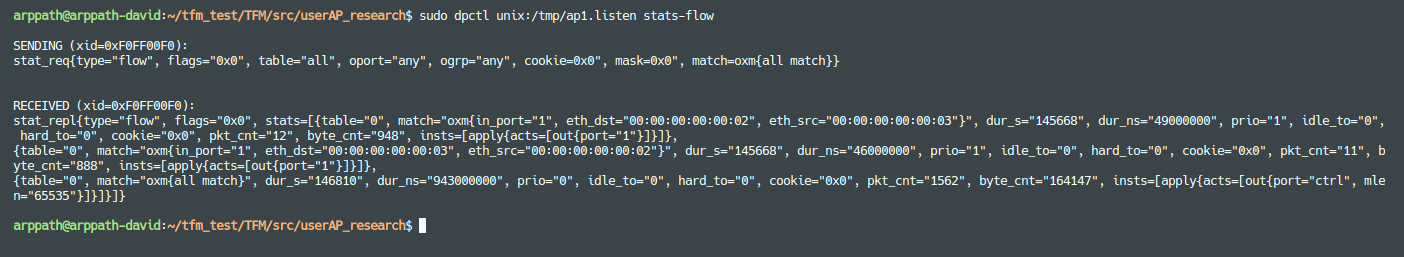
\includegraphics[width=\textwidth]{archivos/img/dev/dpctl_3.png}
    \caption{Información ofuscada de la nueva herramienta \texttt{dpctl}}
    \label{fig:dpctl_3}
\end{figure}

En la figura, se visualiza el comando que se envía al socket UNIX \texttt{unix:/tmp/ap1.listen}, junto con los datos recibidos. Sin embargo, como se mencionó previamente, la información se muestra de manera poco clara o comprensible. Por lo tanto, se requerirá realizar un proceso de análisis y parseo para obtener una visualización más legible de los datos.\\
\\

No obstante, es relevante destacar que esta necesidad no ha sido planteada por primera vez. Un usuario de \gls{bofus} ya había abordado esta cuestión en su momento y realizó una petición en forma de \textit{pull request} en el repositorio, agregando un script en Python para el análisis de la información recibida desde el switch. Dicho script, creado por un desarrollador israelí\footnote{\url{https://github.com/simhond}}, fue escrito en una versión anterior de Python (Python 2.7). Dado que el script podría mejorarse en varios aspectos dado que el JSON resultante no está correctamente formado, y las expresiones regulares no funcionaban en todos los casos. Después de implementar el parser, la salida obtenida del mismo comando se puede apreciar en la Figura \ref{fig:dpctl_4}.


% fig
\begin{figure}[ht]
    \centering
    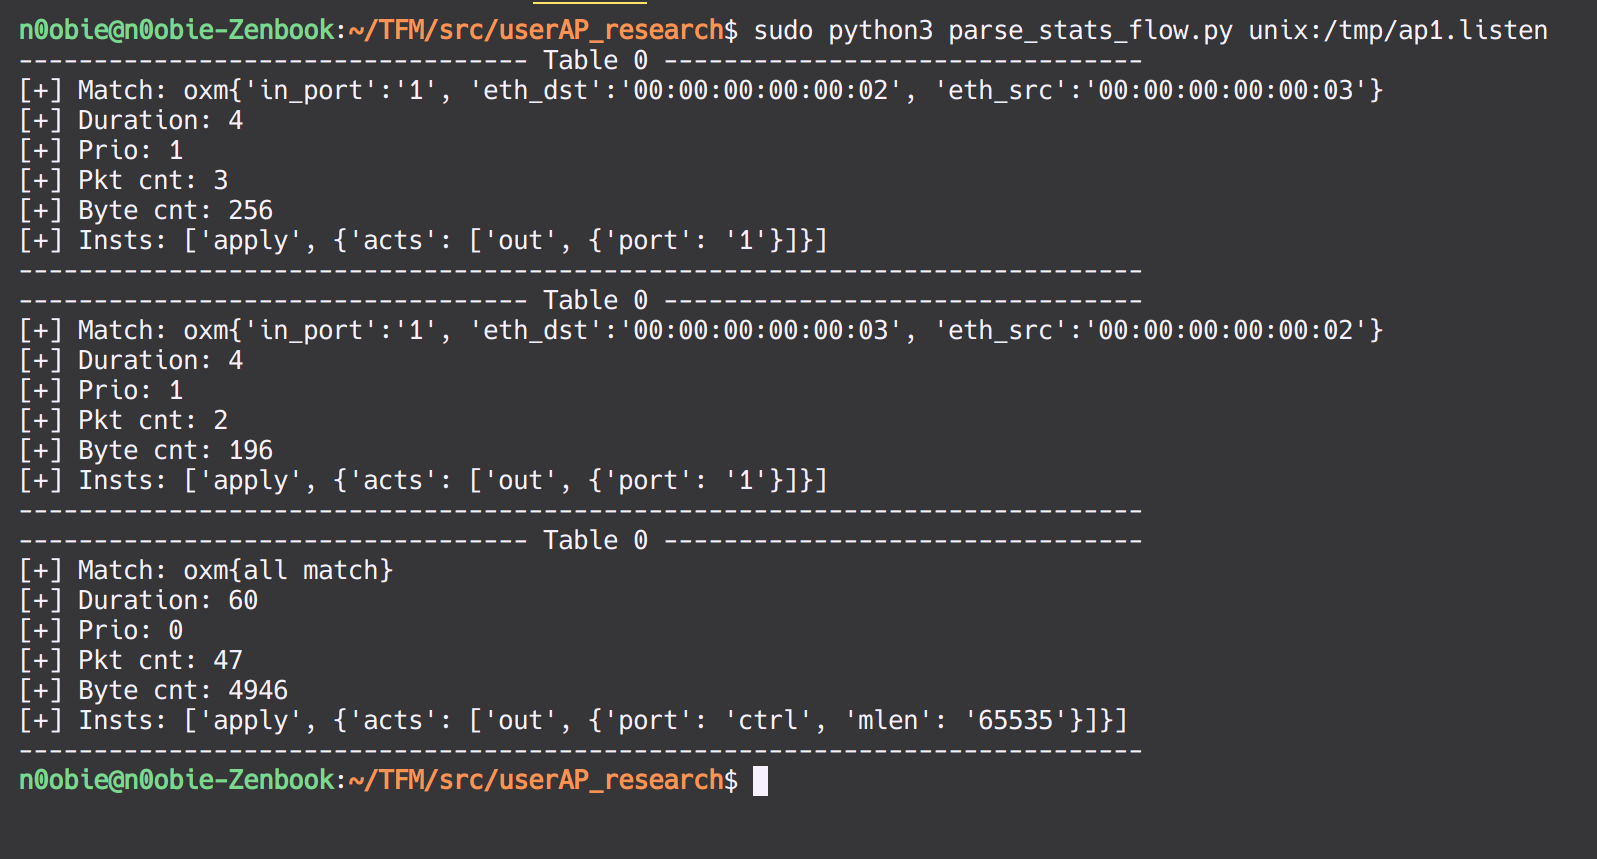
\includegraphics[width=\textwidth]{archivos/img/dev/dpctl_4.png}
    \caption{Resultado del parser la nueva herramienta \texttt{dpctl}}
    \label{fig:dpctl_4}
\end{figure}

\subsection{Rollback a la herramienta \texttt{dpctl}}

La segunda opción consiste en adaptar la herramienta antigua. Para lograr esto, se debe acceder al repositorio de la herramienta anterior llamada ``dpctl" y compilarla sobre la herramienta nueva desarrollada por Eder. A continuación, se proporciona el enlace\footnote{\url{https://github.com/mininet/openflow/tree/master}} al repositorio de la herramienta antigua. Los pasos a seguir son los siguientes, considerando una instalación limpia de Mininet, haciendo referencia al escenario utilizado\footnote{\url{https://github.com/davidcawork/TFM/tree/main/src/scenarios/mininet}}.

\begin{lstlisting}[language= bash, style=Consola, caption={Instalación de las dependencias de la nueva versión de dpctl},label=code:dpctlold1]
    # Tenemos que clonar el repositorio de Openflow indicado anteriormente
    git clone https://github.com/mininet/openflow.git

    # Hacemos un install de las deps
    sudo apt install git autotools-dev pkg-config libc6-dev
\end{lstlisting}
\vspace{0.5cm}


Una vez que se ha clonado el repositorio de OpenFlow de Standford con la versión 1.0 de OpenFlow, se deben instalar las dependencias generales necesarias para compilar el repositorio desde el código fuente. Cabe mencionar que sería más apropiado construir exclusivamente la herramienta y no todo el repositorio, incluyendo el controlador y la implementación 1.0 de OpenFlow. Sin embargo, para realizar una prueba conceptual, será suficiente. Una vez que se tienen las dependencias necesarias instaladas, podemos proceder hacer la contrucción de la herramienta. A continuación, en el bloque de Código \ref{code:dpctlold2}, se indican los pasos para hacer un build desde el source:

\begin{lstlisting}[language= bash, style=Consola, caption={Construcción de la nueva versión de dpctl},label=code:dpctlold2]
    # Entramos
    cd openflow

    # Booteamos y configuramos 
    # (a.k.a pre-checking de que tenemos todas las herramientas para hacer el make)
    ./boot.sh
    ./configure

    # Build :)
    make

    # E instalamos para que el binari oen path de dpctl sea este ultimo
    sudo make install
\end{lstlisting}
\vspace{0.5cm}


Una vez se ha instalado la herramienta, cuando se ejecute la ayuda del binario \texttt{dpctl -h}, se tendría que apreciar el contenido de la Figura \ref{fig:dpctl_5}. Para hacer una prueba de concepto, se ha levantado una topología de ejemplo con Mininet, con \texttt{userSwitchs}, y se ha comprobado como ahora la herramienta de control, si es capaz de extraer los flujos sin ningún tipo de problema (Ver Figura \ref{fig:dpctl_5}).
\newpage

% fig
\begin{figure}[ht!]
    \centering
    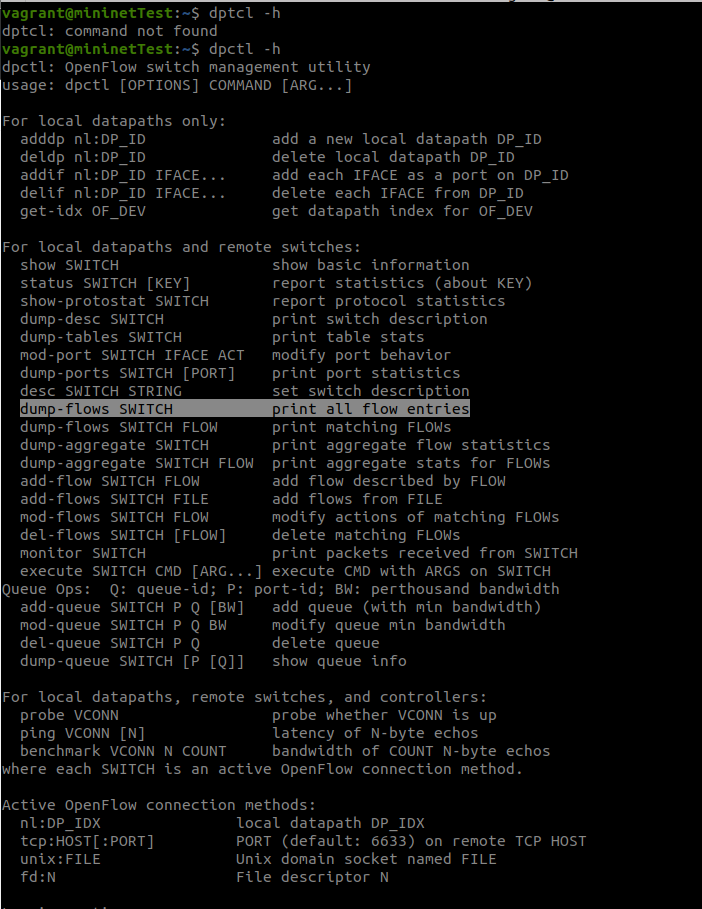
\includegraphics[width=0.8\textwidth]{archivos/img/dev/dpctl_5.png}
    \caption{\textit{Rollback} a la nueva herramienta \texttt{dpctl}}
    \label{fig:dpctl_5}
\end{figure}

\newpage

% fig
\begin{figure}[ht!]
    \centering
    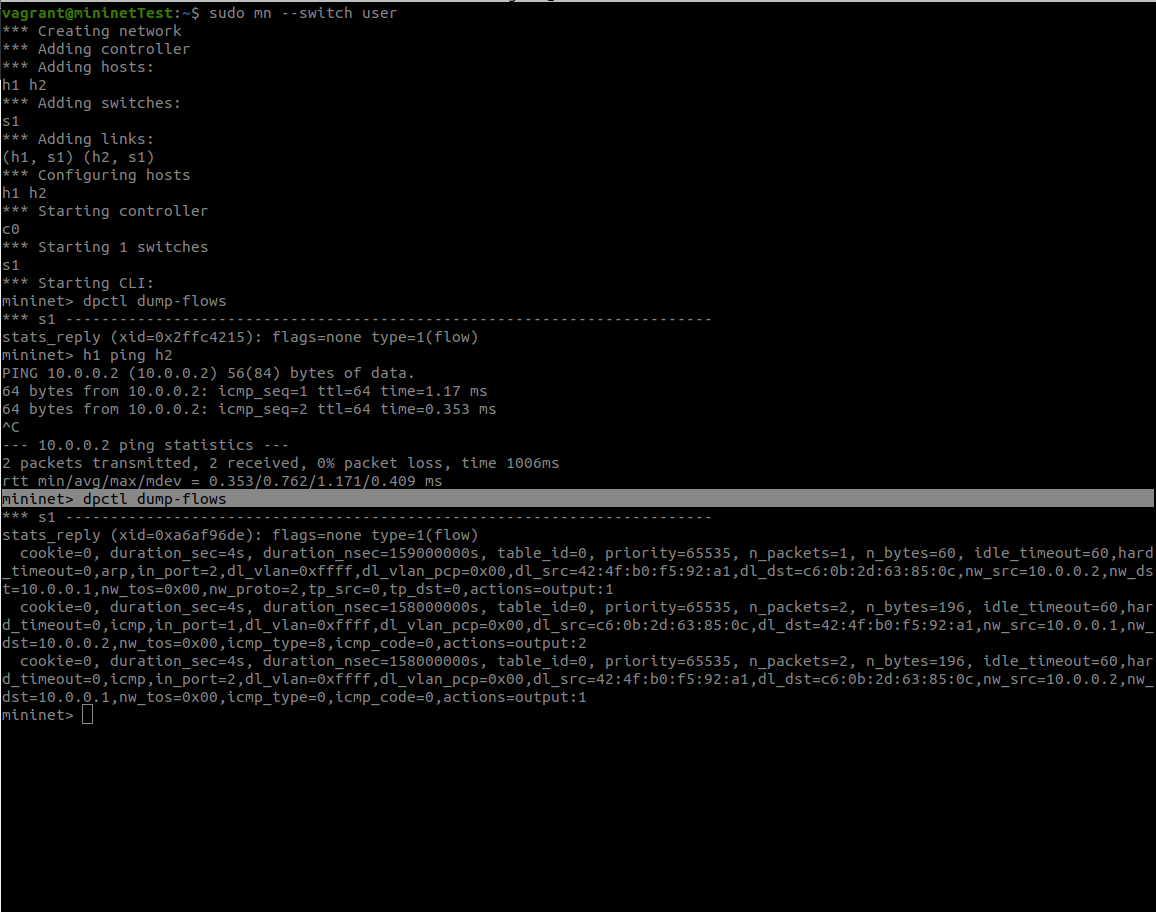
\includegraphics[width=\textwidth]{archivos/img/dev/dpctl_6.png}
    \caption{Funcionamiento de la herramienta antigua sobre Mininet}
    \label{fig:dpctl_6}
\end{figure}